\icode{E-MM-CA-L3-261014-002}
如图所示，足够大的光滑水平地面上静置一质量\(m_2 =\)\,\qty{6}{kg}、带\(\sfrac{1}{4}\)光滑圆弧轨道的滑块\(B\)，圆弧轨道的底端与地面相切，半径\(R =\)\,\qty{0.9}{m}；质量\(m_1 =\)\,\qty{3}{kg}的小球\(A\)从滑块\(B\)顶端正上方\(h =\)\,\qty{0.5}{m}高处由静止落下，无碰撞地进入圆弧轨道，小球\(A\)可视为质点，不计空气阻力，取重力加速度大小\(g =\)\,\qty{10}{m/s^2}。求：
\begin{enumerate}
	\item 小球\(A\)进入圆弧轨道时的动能；
	\item 滑块\(B\)对小球\(A\)做的功\(W\)。
\end{enumerate}

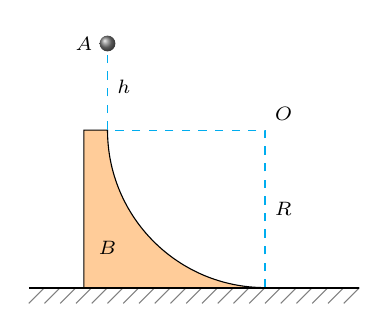
\begin{tikzpicture}[font=\scriptsize]
	\draw[fill=orange!40] (0,0) arc(-90:-180:2)--(-2.3,2)--(-2.3,0);
	\draw[dashed,cyan] (0,0)--node[right,black]{\(R\)}(0,2)node[above right,black]{\(O\)}--(-2,2)--node[right,black]{\(h\)}(-2,3.1);
	\shade[ball color=gray] (-2,3.1) circle(.1);
	\foreach \x in {-3,-2.8,...,1}
		\draw[gray] (\x,-.2)--++(.2,.2);
	\draw[thick] (-3,0)--(1.2,0);
	\node at(-2.3,3.1){\(A\)};
	\node at(-2,.5){\(B\)};
\end{tikzpicture}
\begin{answer}
    （1）\qty{15}{J}（2）\qty{-14}{J}
\end{answer}
